\documentclass[11pt]{article}
\usepackage[utf8]{inputenc}	% Para caracteres en español
\usepackage{amsmath,amsthm,amsfonts,amssymb,amscd}
\usepackage{multirow,booktabs}
\usepackage[table]{xcolor}
\usepackage{fullpage}
\usepackage{lastpage}
\usepackage{enumitem}
\usepackage{fancyhdr}
\usepackage{mathrsfs}
\usepackage{wrapfig}
\usepackage{setspace}
\usepackage{calc}
\usepackage{multicol}
\usepackage{cancel}
\usepackage[retainorgcmds]{IEEEtrantools}
\usepackage[margin=1cm]{geometry}
\usepackage{amsmath}
\newlength{\tabcont}
\setlength{\parindent}{0.0in}
\setlength{\parskip}{0.05in}
\usepackage{empheq}
\usepackage{framed}
\usepackage[most]{tcolorbox}
\usepackage{xcolor}
\usepackage{graphicx}
\usepackage{listings}
% -- Basic formatting
\usepackage[utf8]{inputenc}
\usepackage[english]{babel}
\usepackage{times}
\usepackage{caption}
\usepackage{subcaption}
\usepackage{placeins}
\setlength{\parindent}{0pt}
\usepackage{indentfirst}% -- Defining colors:
\usepackage[dvipsnames]{xcolor}
\definecolor{codegreen}{rgb}{0,0.6,0}
\definecolor{codegray}{rgb}{0.5,0.5,0.5}
\definecolor{codepurple}{rgb}{0.58,0,0.82}
\definecolor{backcolour}{rgb}{0.95,0.95,0.92}% Definig a custom style:
\lstdefinestyle{mystyle}{
    backgroundcolor=\color{backcolour},   
    commentstyle=\color{codepurple},
    keywordstyle=\color{NavyBlue},
    numberstyle=\tiny\color{codegray},
    stringstyle=\color{codepurple},
    basicstyle=\ttfamily\footnotesize\bfseries,
    breakatwhitespace=false,         
    breaklines=true,                 
    captionpos=t,                    
    keepspaces=true,                 
    numbers=left,                    
    numbersep=5pt,                  
    showspaces=false,                
    showstringspaces=false,
    showtabs=false,                  
    tabsize=2
}% -- Setting up the custom style:
\lstset{style=mystyle}
\lstset{
  style=mystyle,
  framexleftmargin=3.5mm,
  rulesepcolor=\color{black},
  linewidth=0.6\linewidth,
  xleftmargin=12pt,
  aboveskip=12pt,
  belowskip=12pt
}
\colorlet{shadecolor}{orange!15}
\parindent 0in
\parskip 1pt
\geometry{margin=1in, headsep=0.25in}
\theoremstyle{definition}
\newtheorem{defn}{Definition}
\newtheorem{reg}{Rule}
\newtheorem{exer}{Exercise}
\newtheorem{note}{Note}
\graphicspath{ {./images/} }
\begin{document}
\setcounter{section}{0}
\title{MIE223 Lecture Notes}

\thispagestyle{empty}

\begin{center}
{\LARGE \bf Sentiment Analysis}\\
{\large MIE223}\\
Winter 2025
\end{center}
\section{Sentiment Analysis}
\subsection{Positive or negative movie review?}
\begin{itemize}
  \item unbelievably disappointing
  \item Full of zany characters and richly applied satire, and some
  great plot twists
  \item this is the greatest screwball comedy ever filmed
  \item It was pathetic. The worst part about it was the boxing
  scenes.
\end{itemize}

\begin{verbatim}
  How do we find the sentiment of a review? you can automatically 
  extract common tokens and phrases from the reviews and use them 
  to determine the sentiment of the review. We use phrase chunking 
  to get key phrases. use entailment to determine if a sentence 
  is relevant to a specific key phrase.
  determine whether phrase is positive or negative
  called polarity analysis.
\end{verbatim}

\subsection{Twitter sentiment versus Gallup Poll of
Consumer Confidence}
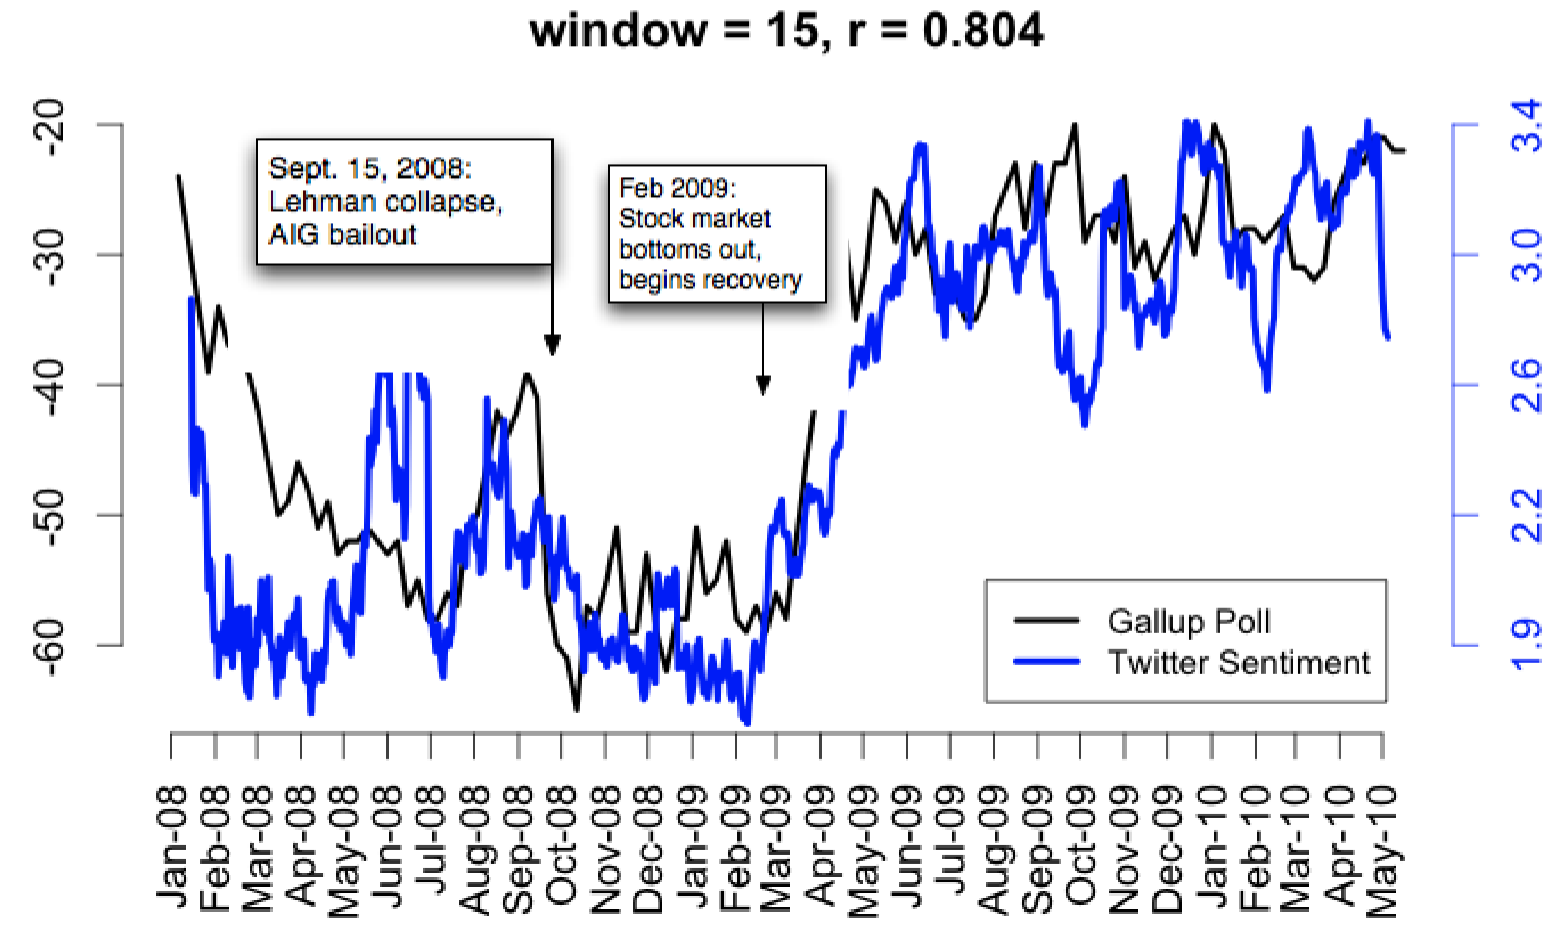
\includegraphics[width=\textwidth/2]{7.png}
\begin{itemize}
  \item gallup poll can be used to survey public opinion
  \item twitter sentiment can be used to predict public opinion
\end{itemize}

\subsection{Twitter sentiment:}
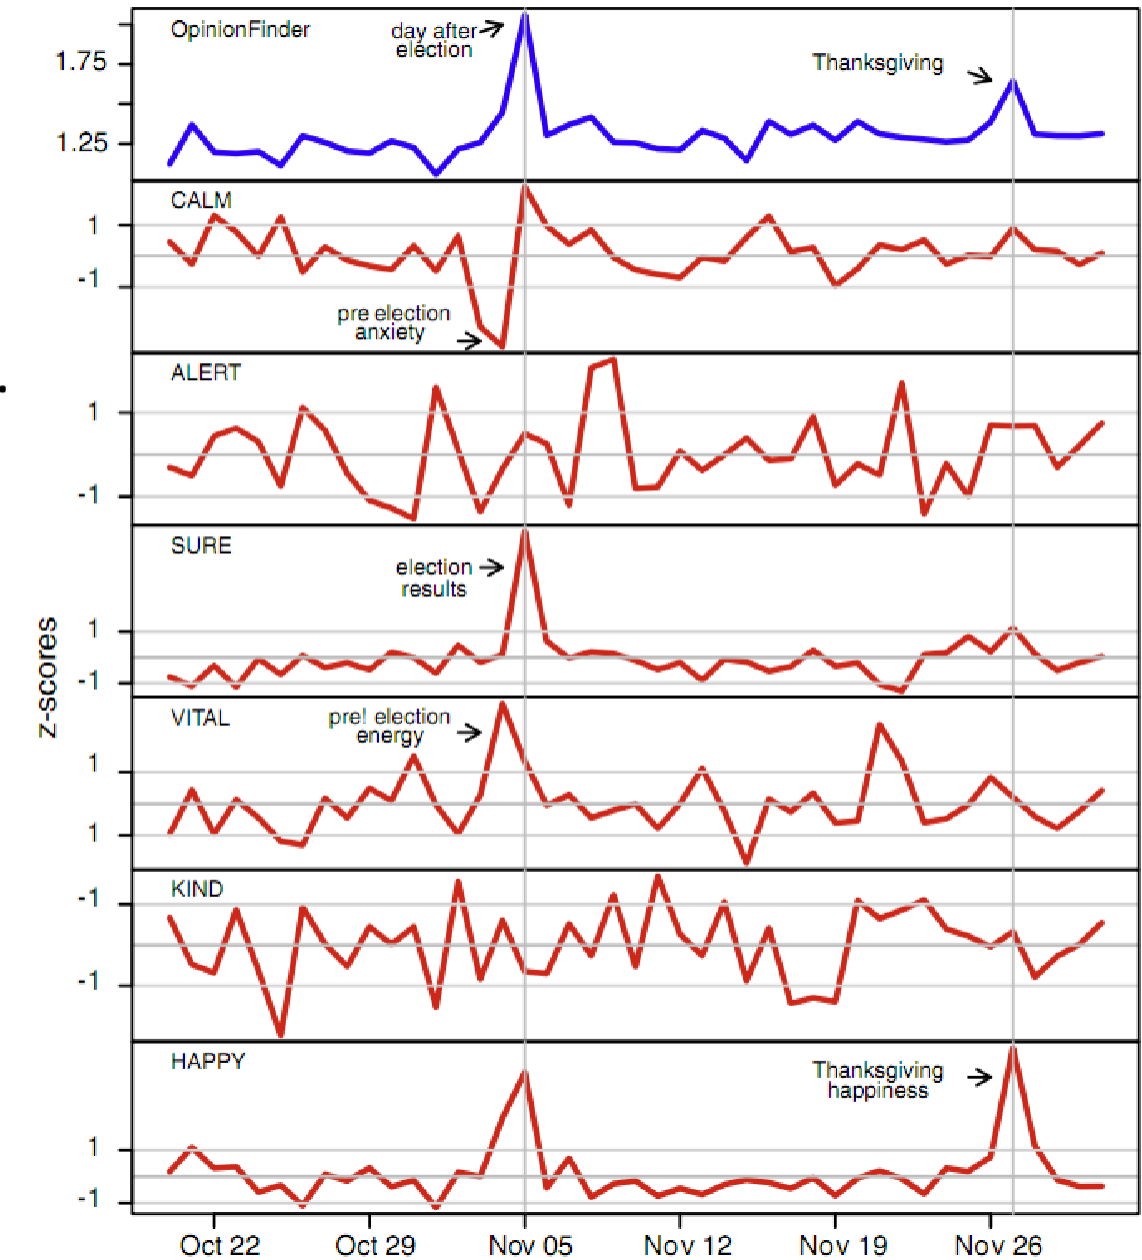
\includegraphics[width=\textwidth/2]{8.png}
\begin{itemize}
  \item CALM predicts
  DJIA 3 days
  later, Twitter predicts the stock market shifts 2-6 days later
  \item At least one
  current hedge
  fund uses this
  algorithm
\end{itemize}
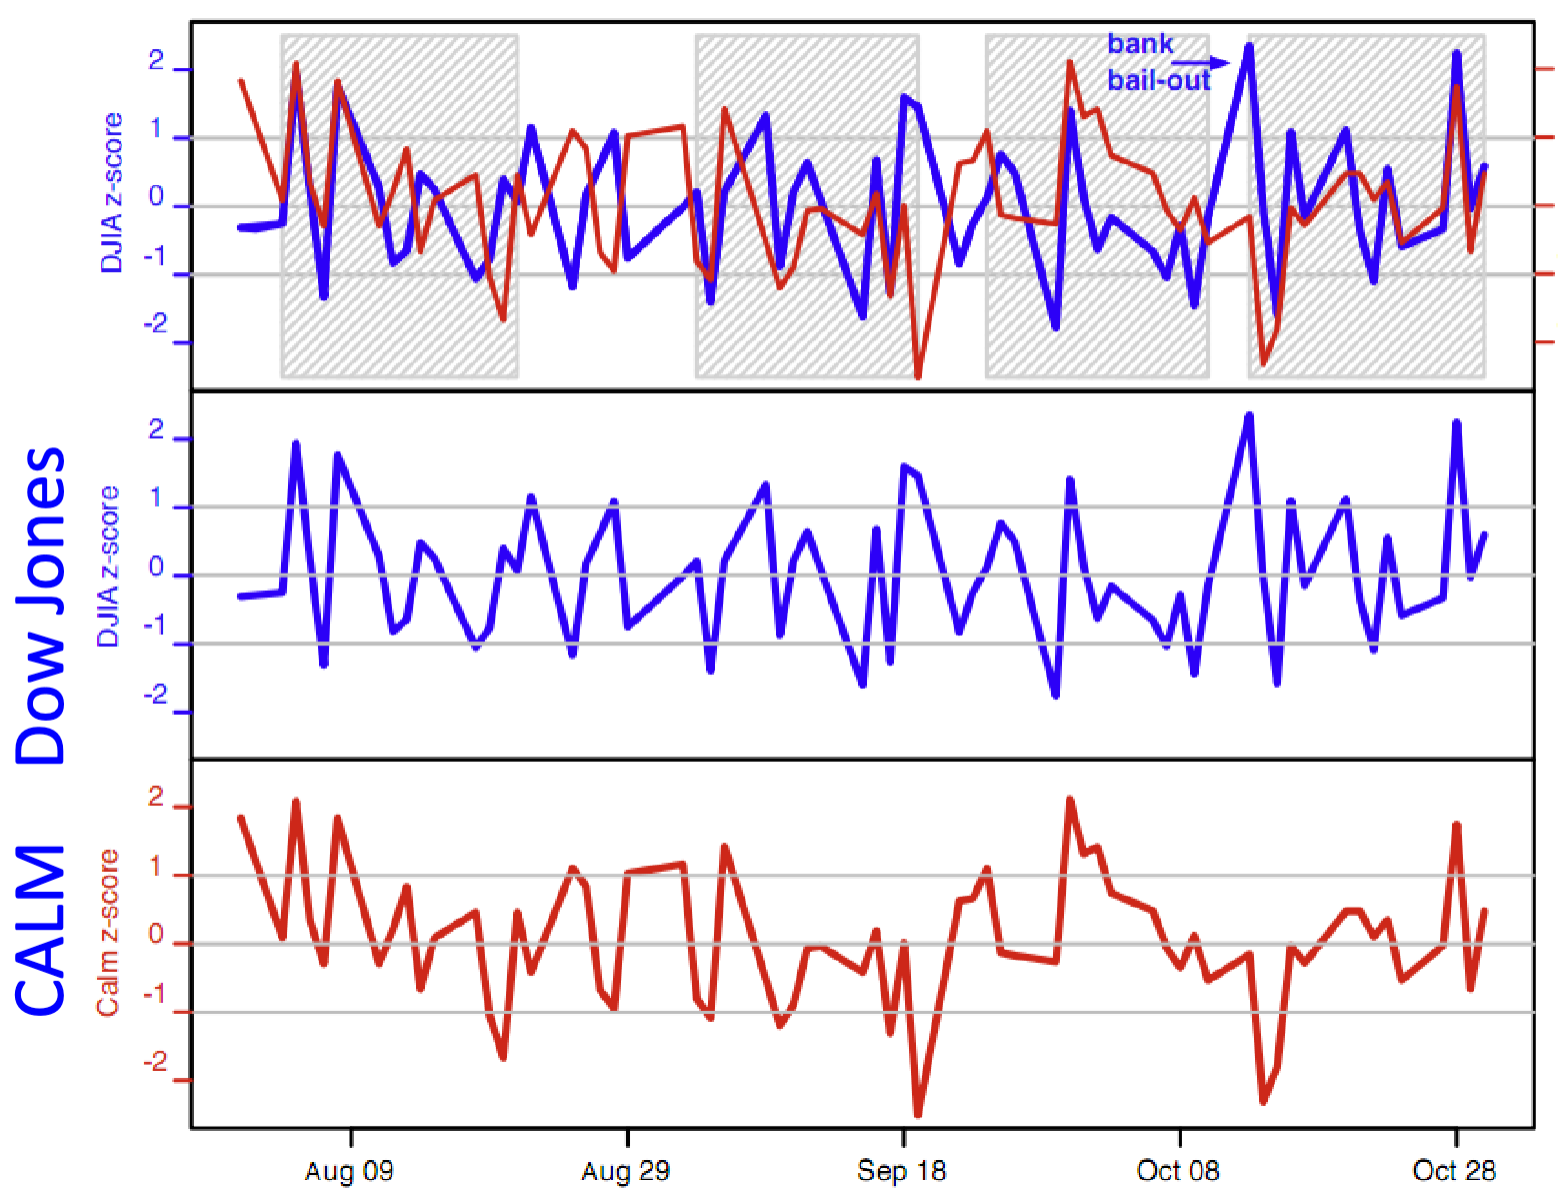
\includegraphics[width=\textwidth/2]{9.png}
\begin{itemize}
  \item an efficient market makes use of information
  \item twitter sentiment can be used to predict stock prices
  \item the results are terrible
  \item ideas are good, nuanced emotions can influence the stock market
  \item different events give rise to different emotions which can be measured
\end{itemize}

\subsection{Beware: Spurious Correlations}
\begin{itemize}
  \item data matching correlations are similar but not true
\end{itemize}

\subsection{Target Sentiment on Twitter}
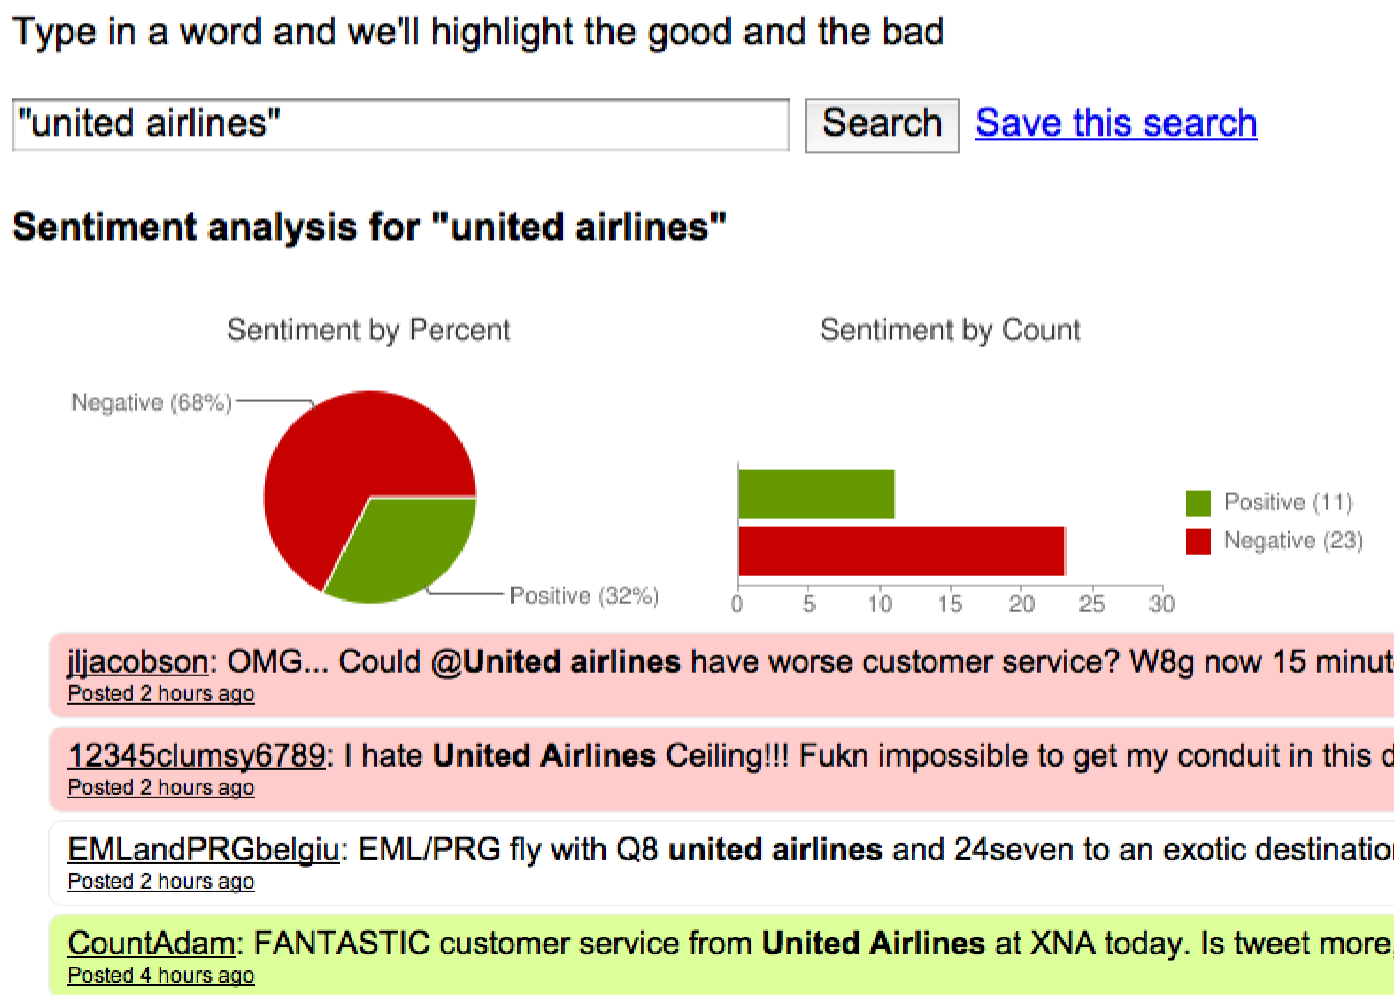
\includegraphics[width=\textwidth/2]{11.png}

\subsection{Sentiment analysis has many other names}
\begin{itemize}
  \item Opinion extraction
  \item Opinion mining
  \item Sentiment mining
  \item Subjectivity analysis
\end{itemize}

\subsection{Why sentiment analysis?}
\begin{itemize}
  \item Movie: is this review positive or negative?
  \item Products: what do people think about the new iPhone?
  \item Public sentiment: how is consumer confidence? Is despair
  increasing?
  \item Politics: what do people think about this candidate or issue?
  \item Prediction: predict election outcomes or market trends from
  sentiment
\end{itemize}

\subsection{Scherer Typology of Affective States}
\begin{itemize}
  \item Emotion: brief organically synchronized ... evaluation of a major event
  \begin{itemize}
  \item angry, sad, joyful, fearful, ashamed, proud, elated
  \end{itemize}
  \item Mood: diffuse non-caused low-intensity long-duration change in subjective feeling
  \begin{itemize}
    \item cheerful, gloomy, irritable, listless, depressed, buoyant
  \end{itemize}
  \item Interpersonal stances: affective stance toward another person in a specific interaction
  \begin{itemize}
    \item friendly, flirtatious, distant, cold, warm, supportive, contemptuous
  \end{itemize}
  \item Attitudes: enduring, affectively colored beliefs, dispositions towards objects or persons
  \begin{itemize}
    \item liking, loving, hating, valuing, desiring
  \end{itemize}
  \item Personality traits: stable personality dispositions and typical behavior tendencies
  \begin{itemize}
    \item nervous, anxious, reckless, morose, hostile, jealous
  \end{itemize}
\end{itemize}
\begin{note}
  Majority of review sentiment focuses on attitudes. Public mood predicts stock market.
\end{note}

\subsection{Sentiment Analysis}
\begin{itemize}
  \item Sentiment analysis is the detection of \textbf{attitudes}
  \item “enduring, affectively colored beliefs, dispositions towards objects or persons”
\end{itemize}
\begin{enumerate}
  \item Holder (source) of attitude
  \item Target (aspect) of attitude
  \item Type of attitude
  \begin{itemize}
    \item From a set of types like, love, hate, value, desire, etc.
    \item Or (more commonly) simple weighted polarity: 
    \begin{itemize}
      \item positive, negative, neutral, together with strength
    \end{itemize}
  \end{itemize}
  \item Text containing the attitude like sentence or entire document
  \item Coreference resolution: who is talking about what?
\end{enumerate}
\begin{itemize}
  \item Simplest task:
  \begin{itemize}
    \item Is the attitude of this text positive or negative?
  \end{itemize}
  \item More complex:
  \begin{itemize}
    \item Rank the attitude of this text from 1 to 5
  \end{itemize}
  \item Advanced:
  \begin{itemize}
    \item Detect the target, source, or complex attitude types
  \end{itemize}
\end{itemize}

\section{Text Processing and
Sentiment Classifier
Limitations}
\subsection{Sentiment Classification in Movie Reviews}
\begin{itemize}
  \item Polarity detection:
  \begin{itemize}
    \item Is an IMDB movie review positive or negative?
  \end{itemize}
\end{itemize}

\subsection{IMDB data in the Pang and Lee database}
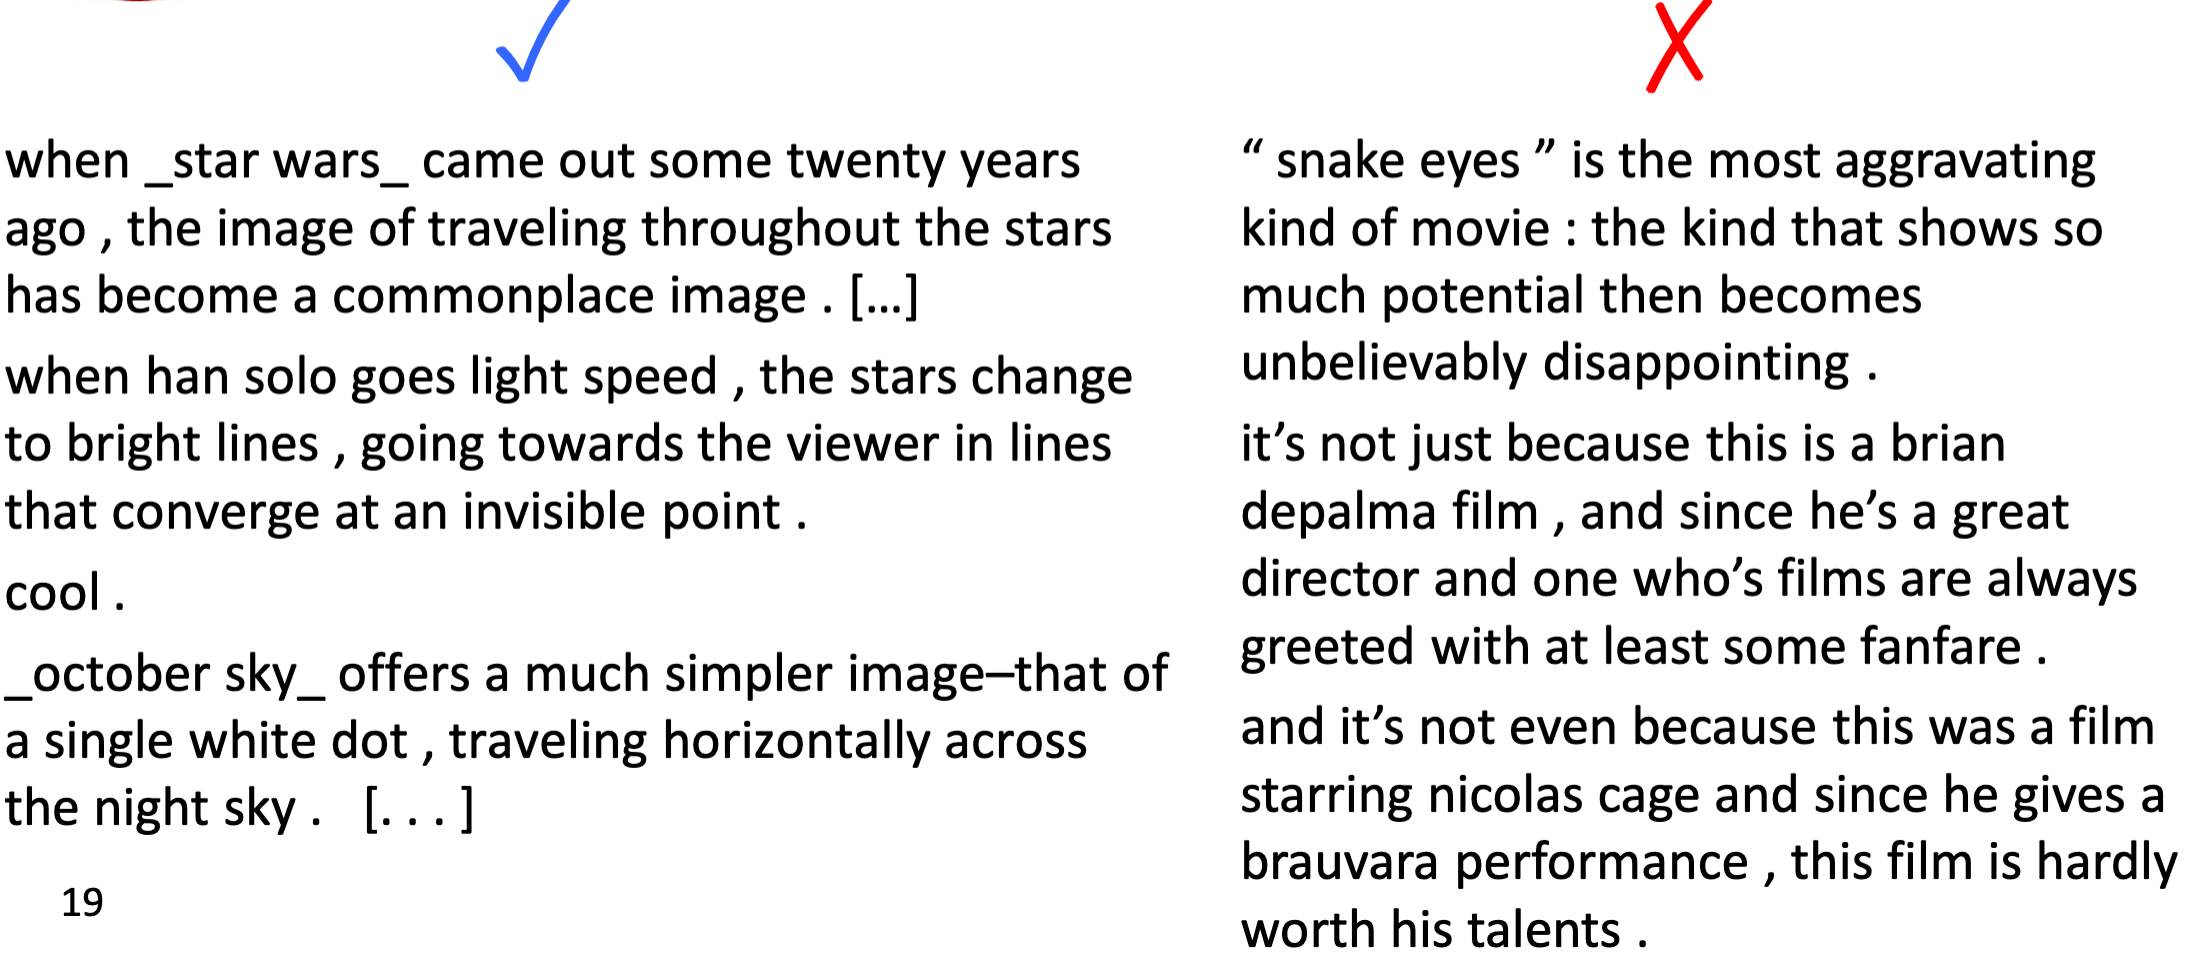
\includegraphics[width=\textwidth]{12.png}

\subsection{Sentiment Analysis and Prediction}
\begin{itemize}
  \item Sentiment-aware tokenization
  \begin{itemize}
    \item Important if text analysis should be sensitive to sentiment
  \end{itemize}
\end{itemize}
\begin{itemize}
  \item Prediction using different classifiers / regressors
  \begin{itemize}
    \item Could learn with Naïve Bayes, Logistic Regression, SVM
  \end{itemize}
  \begin{itemize}
    \item Vader is an off-the-shelf tool for predicting sentiment
    \item Actually a regressor, predicts strength of polarity [-1,+1]
    \item +1 = Most positive, -1 = Most negative, 0 = Neutral
  \end{itemize}
\end{itemize}

\subsection{Sentiment Tokenization Issues}
Let’s consider tokenization
text analysis should be
sensitive to sentiment

\begin{itemize}
  \item Capitalization
  \begin{itemize}
    \item Preserve capital letters
    \item Why?
  \end{itemize}
  \item Emoticons (useful to express emotion)
  \item Useful code Regex
\end{itemize}

\includegraphics[width=\textwidth/2]{13.png}

\subsection{Classification Results}
\begin{itemize}
  \item Trained classifier achieves 92.1\% accuracy on movies
  \begin{itemize}
    \item Off-the-shelf Vader would do well: around 80-85\% accuracy
  \end{itemize}
\end{itemize}
\begin{itemize}
  \item Need to train a classifier per domain for best results
  \begin{itemize}
    \item Scary movie = good!
    \item Scary hotel = bad!
    \item Hotel with “thin walls”?  
  \end{itemize}
  \item Vader would deem scary bad even though it may be good for movies
\end{itemize}

\subsection{Classifiers don’t capture everything}
Subtlety:

\begin{itemize}
  \item Perfume review in Perfumes: the Guide:
  \begin{itemize}
    \item “If you are reading this because it is your darling fragrance,
    please wear it at home exclusively, and tape the windows
    shut.”
    \item not a good review but has positive adjectives
  \end{itemize}
  \item Dorothy Parker on Katherine Hepburn
  \begin{itemize}
    \item "She runs the gamut of emotions from A to B”
    \item bad statement but no negative words
  \end{itemize}
\end{itemize}

\begin{itemize}
  \item Word interactions:
  \begin{itemize}
    \item Raising taxes = bad
    \item Raising salaries = good
    \item Lowering taxes = good
    \item Lowering salaries = bad
  \end{itemize}
  \item A solution? Adjective*Noun where... word interactions
  \begin{itemize}
    \item Raising=+1, Lowering=-1, Taxes=-1, Salaries=+1
    \item Also supports Adverb*Adjective: very(+2) happy (+1), very (+2) sad (-1)
  \end{itemize}
\end{itemize}

\begin{note}
  the holder and target matter as well. here the opinion holder is assumed to be an individual, but how would this change if the opinon holder was a government or organization?
\end{note}

\subsection{Thwarted Expectations
and Ordering Effects}
\begin{itemize}
  \item “This film should be brilliant. It sounds like a great plot, the actors are first
  grade, and the supporting cast is good as well, and Stallone is attempting to
  deliver a good performance. However, it can’t hold up.”
  \item Well as usual Keanu Reeves is nothing special, but surprisingly, the very
  talented Laurence Fishbourne is not so good either, I was surprised
\end{itemize}
\begin{note}
  many good things but one bad thing turns the entire thing negative
\end{note}

\subsection{Sarcasm}
\begin{itemize}
  \item Josef Stalin might enjoy this movie.
  \item As exciting as watching the grass grow.
  \item This movie should win flop of the year.
  \item I wondered whether I had checked into the Bates Motel.
\end{itemize}

\section{Sentiment Lexicons}
\subsection{Disagreements between polarity lexicons}
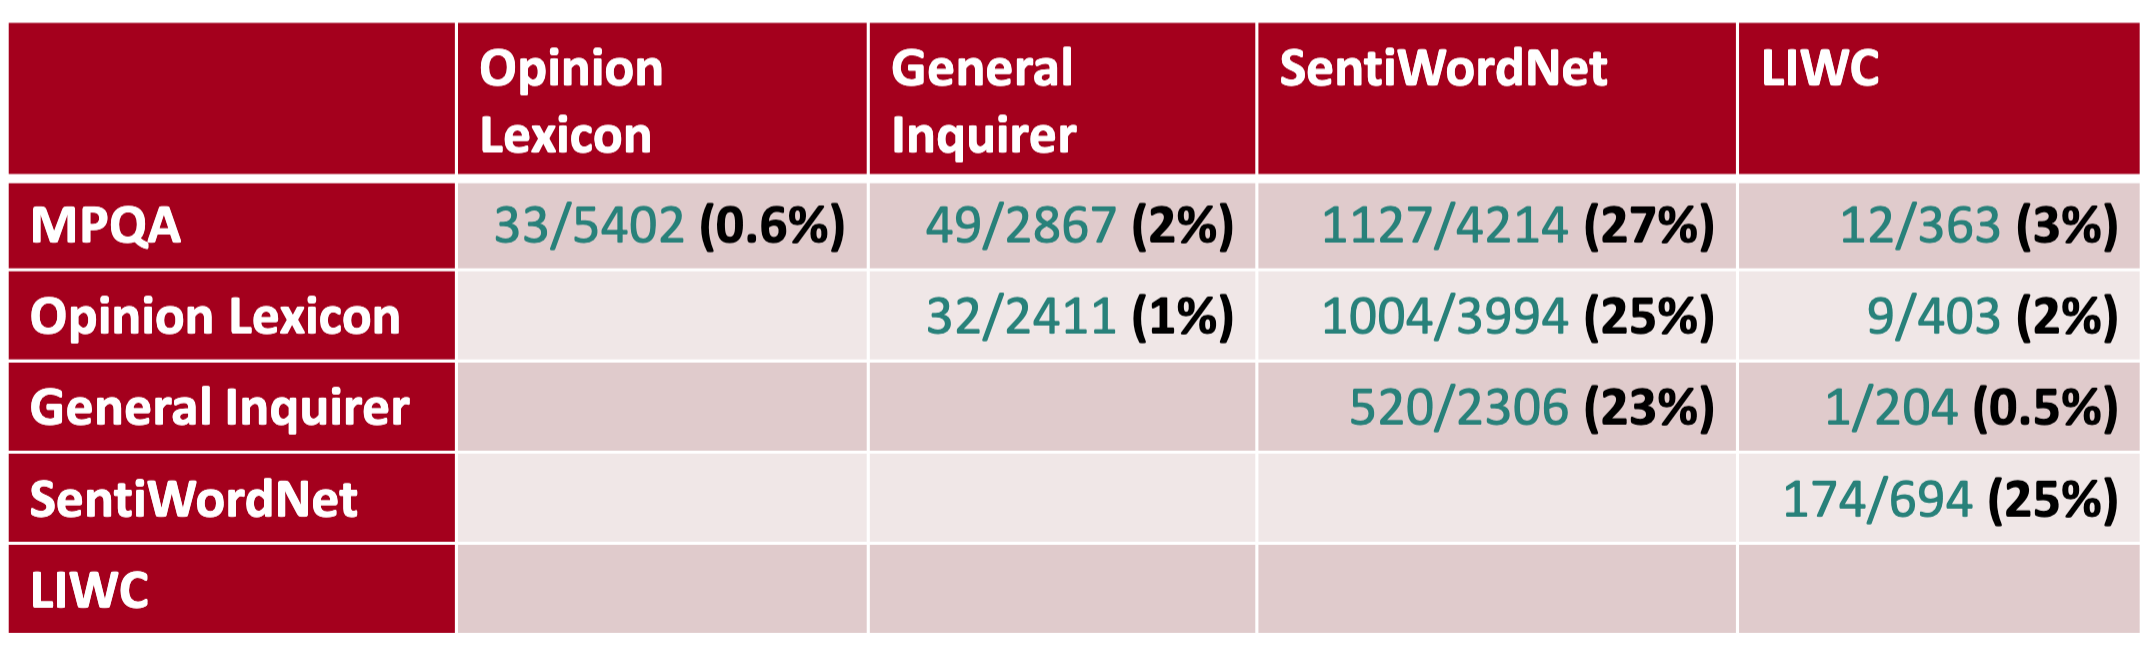
\includegraphics[width=\textwidth]{14.png}

\section{Automatic Polarity
Analysis (with PMI)}

\subsection{Analyzing the polarity of each word in IMDB}
\begin{itemize}
  \item How likely is each word to appear in each sentiment class?
  \item Count(“bad”) in 1-star, 2-star, 3-star, etc.
  \item But can’t use raw counts:
  \item Instead, likelihood:
  \item Make them comparable between words
  \item Scaled likelihood:
\end{itemize}
\begin{equation}
  likelihood (P(w|c)) = \frac{f(w|c)}{\sum_{w \in c} f(w|c)}
\end{equation}
\begin{equation}
  \text{Scaled likelihood} = \frac{P(w|c)}{P(w)}
\end{equation}
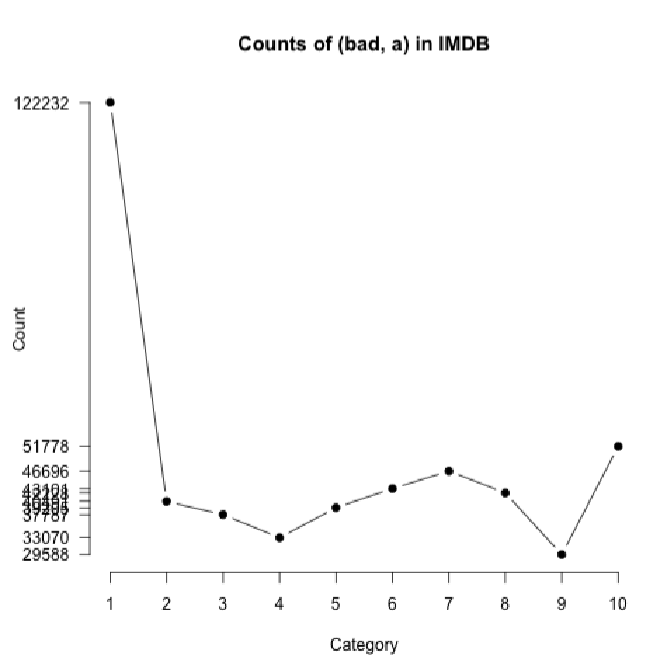
\includegraphics[width=\textwidth/4]{15.png}
\begin{verbatim}
  how often does "bad" show up when pertaining to ratings
  peak at 7 and 10 due to "its not bad" or sheer number of 7 and 10 
  ratings
\end{verbatim}


\subsection{Analyzing the polarity of each word in IMDB}
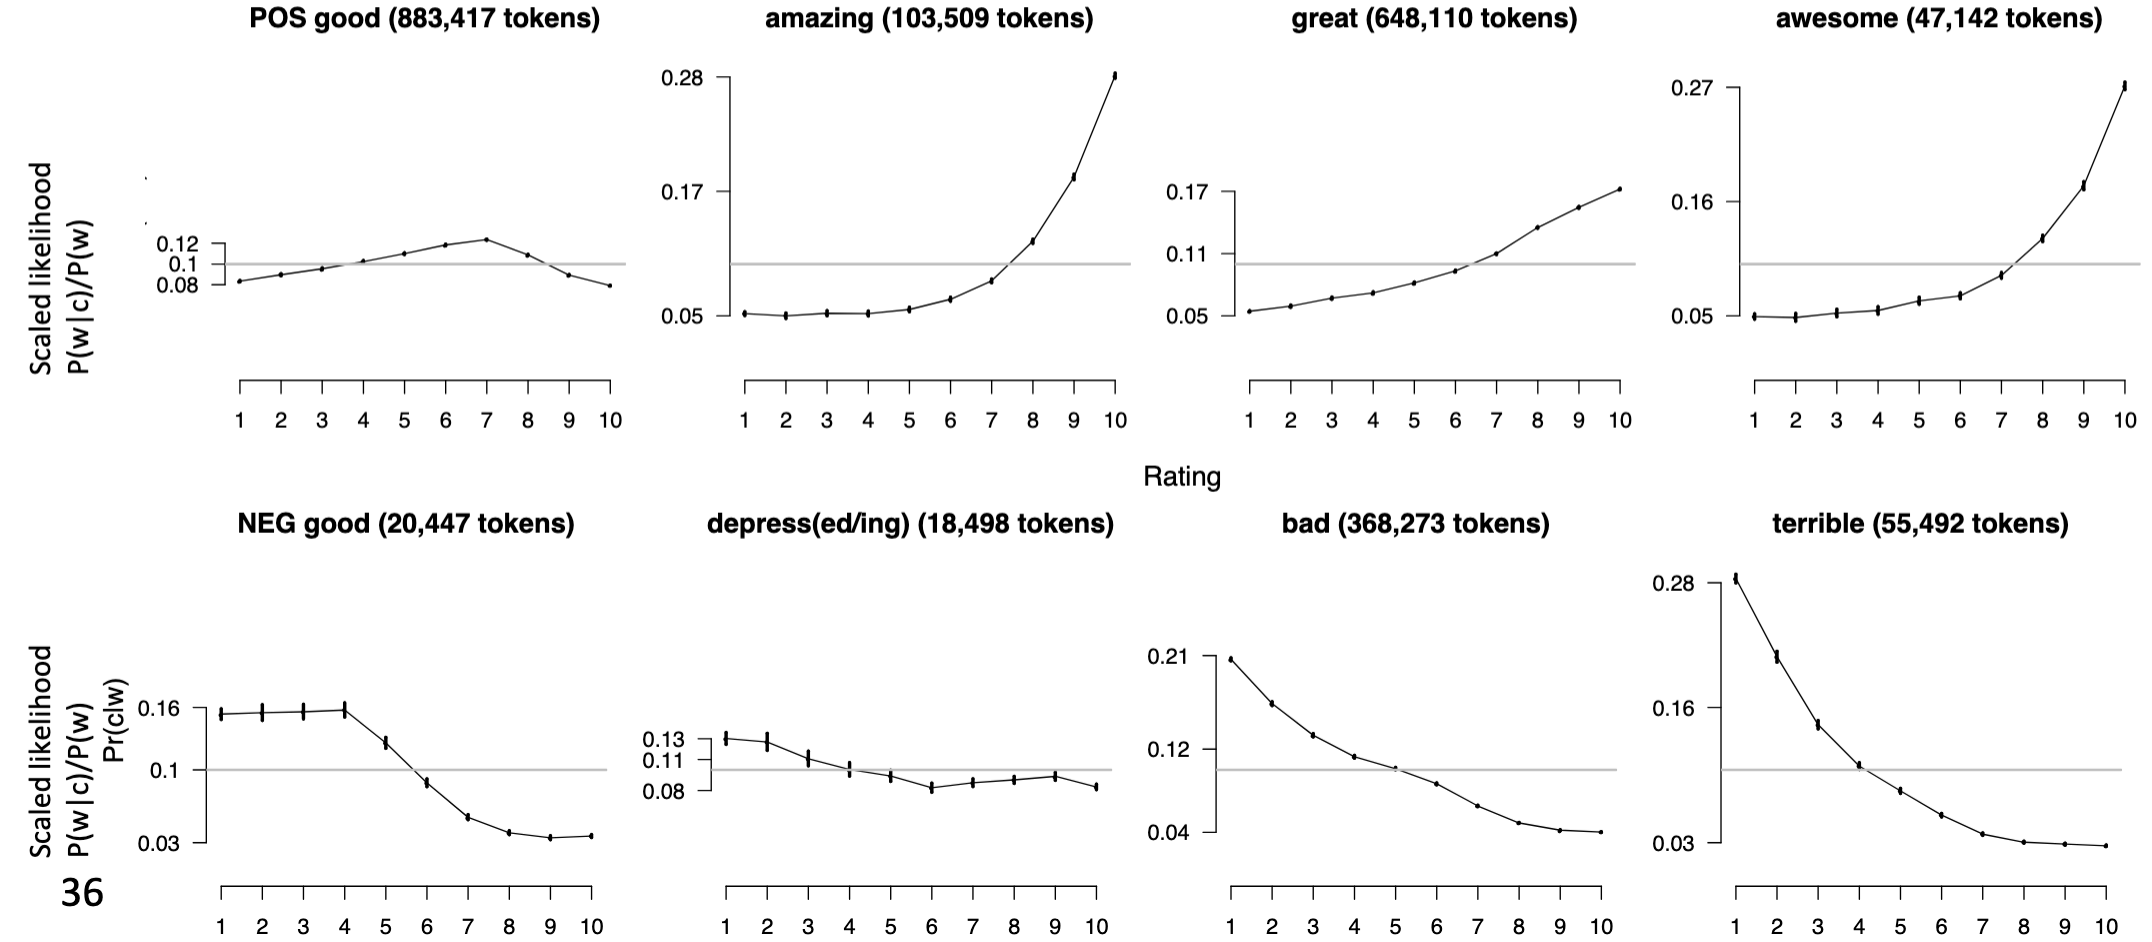
\includegraphics[width=\textwidth]{16.png}

\subsection{Other sentiment feature: Logical negation}
\begin{itemize}
  \item Is logical negation (no, not) associated with negative
  sentiment?
  \item Potts experiment:
  \begin{itemize}
    \item Count negation (not, n’t, no, never) in online reviews
    \item Regress against the review rating
  \end{itemize}
\end{itemize}

\subsection{Potts 2011 Results: More negation in negative sentiment}
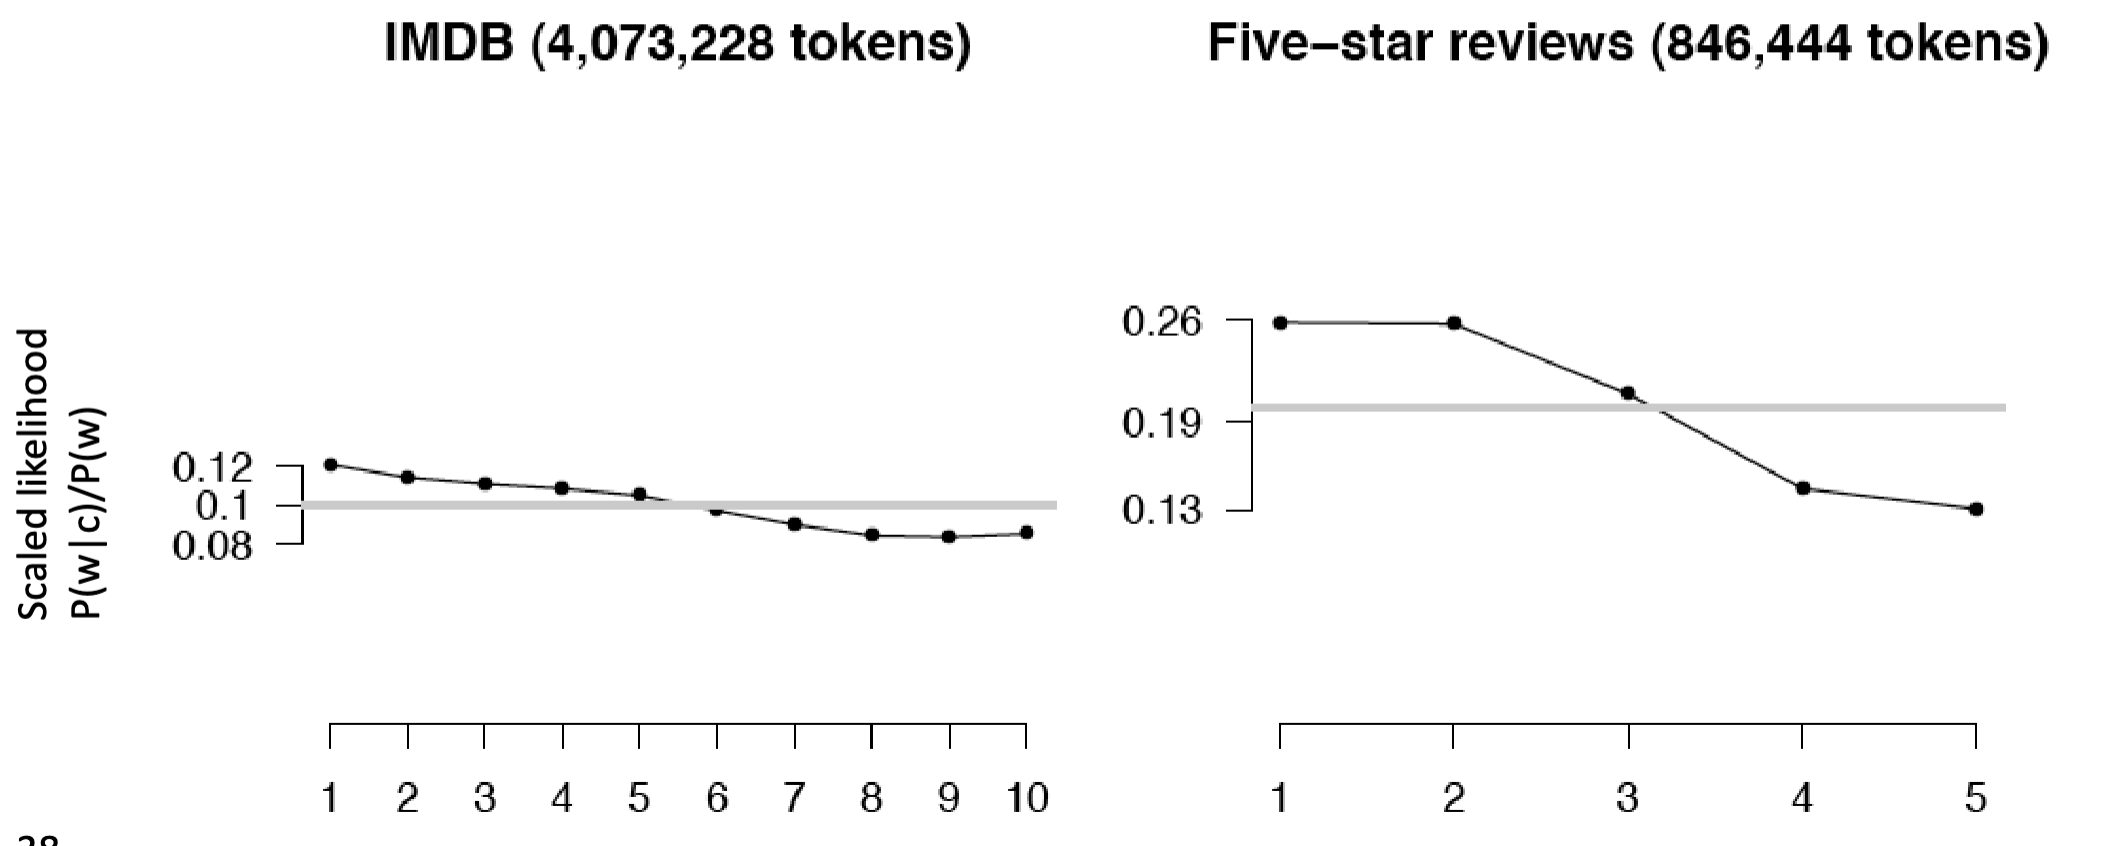
\includegraphics[width=\textwidth]{17.png}

\end{document}